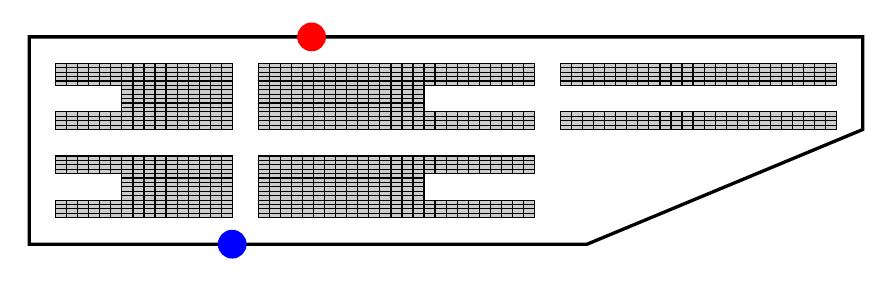
\begin{tikzpicture}[scale=0.07]
%\draw[help lines] (0,0) grid (142,-28);
\colorlet{Grey}{black!20}
%% External perimeter of the harbour
\draw[very thick] (0,0) -- (151.2,0)
	-- (151.2,-16.8) -- (151.2-50,-37.6)
	-- (0,-37.6) -- cycle;
%% Zone top left
\def\a{4.8}
\def\b{-4.8}
\draw[fill=Grey] (\a,\b) -- (\a+32,\b)
	-- (\a+32,\b-12) -- (\a,\b-12)
	-- (\a,\b-12+3.2) -- (\a+12,\b-12+3.2)
	-- (\a+12,\b-4) -- (\a,\b-4) -- cycle;
%
\foreach \x in {0,...,5}
{
	\draw[thin] (\a+2*\x,\b) -- (\a+2*\x,\b-0.8*5);
	\draw[thin] (\a+2*\x,\b-12) -- (\a+2*\x,\b-12+0.8*4);
	\draw[thin] (\a,\b-0.8*\x) -- (\a+32,\b-0.8*\x);
}
\foreach \x in {0,...,10}
{
	\draw[thin] (\a+12+2*\x,\b) -- (\a++12+2*\x,\b-0.8*15);
}
\foreach \x in {0,...,4}
	{\draw[thin] (\a,\b-4-4.8-0.8*\x) -- (\a+32,\b-4-4.8-0.8*\x);}
\foreach \x in {0,...,6}
	{\draw[thin] (\a+12,\b-4-0.8*\x) -- (\a+32,\b-4-0.8*\x);}
%%%%%%%%%%%%%%		
%% Zone bottom left %%
%%%%%%%%%%%%%%
\def\a{4.8}
\def\b{-21.6}
\draw[fill=Grey] (\a,\b) -- (\a+32,\b)
-- (\a+32,\b-11.2) -- (\a,\b-11.2)
-- (\a,\b-11.2+3.2) -- (\a+12,\b-11.2+3.2)
-- (\a+12,\b-3.2) -- (\a,\b-3.2) -- cycle;
%
\foreach \x in {0,...,5}
{
	\draw[thin] (\a+2*\x,\b) -- (\a+2*\x,\b-0.8*4);
	\draw[thin] (\a+2*\x,\b-11.2) -- (\a+2*\x,\b-11.2+0.8*4);
}
\foreach \x in {0,...,10}
{
	\draw[thin] (\a+12+2*\x,\b) -- (\a+12+2*\x,\b-0.8*14);
}
\foreach \x in {0,...,4}
{
	\draw[thin] (\a,\b-3.2-4.8-0.8*\x) -- (\a+32,\b-3.2-4.8-0.8*\x);
	\draw[thin] (\a,\b-0.8*\x) -- (\a+32,\b-0.8*\x);
}
\foreach \x in {0,...,6}
	{\draw[thin] (\a+12,\b-3.2-0.8*\x) -- (\a+32,\b-3.2-0.8*\x);}
%%%%%%%%%%%%%%
%% Zone top central %%
%%%%%%%%%%%%%%
\def\a{41.6}
\def\b{-4.8}
\draw[fill=Grey] (\a,\b) -- (\a+50,\b)
	-- (\a+50,\b-4) -- (\a+50-20,\b-4)
	-- (\a+50-20,\b-4-4.8) -- (\a+50,\b-4-4.8)
	-- (\a+50,\b-12) -- (\a,\b-12) -- cycle;
%
\foreach \x in {0,...,15}
{
	\draw[thin] (\a+2*\x,\b) -- (\a+2*\x,\b-0.8*15);
	\draw[thin] (\a,\b-0.8*\x) -- (\a+30,\b-0.8*\x);
}
\foreach \x in {0,...,10}
{
	\draw[thin] (\a+30+2*\x,\b) -- (\a+30+2*\x,\b-0.8*5);
	\draw[thin] (\a+30+2*\x,\b-8.8) -- (\a+30+2*\x,\b-8.8-0.8*4);
}
\foreach \x in {0,...,5} {\draw[thin] (\a+30,\b-0.8*\x) -- (\a+50,\b-0.8*\x);}
\foreach \x in {0,...,4} {\draw[thin] (\a+30,\b-8.8-0.8*\x) -- (\a+50,\b-8.8-0.8*\x);}
%%%%%%%%%%%%%%%%
%% Zone bottom central %%
%%%%%%%%%%%%%%%%
\def\a{41.6}
\def\b{-21.6}
\draw[fill=Grey] (\a,\b) -- (\a+50,\b)
-- (\a+50,\b-3.2) -- (\a+50-20,\b-3.2)
-- (\a+50-20,\b-3.2-4.8) -- (\a+50,\b-3.2-4.8)
-- (\a+50,\b-11.2) -- (\a,\b-11.2) -- cycle;
%
\foreach \x in {0,...,4} {
	\draw[thin] (\a+30,\b-0.8*\x) -- (\a+50,\b-0.8*\x);
	\draw[thin] (\a+30,\b-8-0.8*\x) -- (\a+50,\b-8-0.8*\x);
}
\foreach \x in {0,...,10}
{
	\draw[thin] (\a+30+2*\x,\b) -- (\a+30+2*\x,\b-0.8*4);
	\draw[thin] (\a+30+2*\x,\b-8) -- (\a+30+2*\x,\b-8-0.8*4);
}
\foreach \x in {0,...,15} {\draw[thin] (\a+2*\x,\b) -- (\a+2*\x,\b-0.8*14);}
\foreach \x in {0,...,14} {	\draw[thin] (\a,\b-0.8*\x) -- (\a+30,\b-0.8*\x);}
%%%%%%%%%%%%%%%%
%%%% Zone top right %%%%
%%%%%%%%%%%%%%%%
\def\a{41.6+4.8+50}
\def\b{-4.8}
\draw[fill=Grey] (\a,\b) -- (\a+50,\b)
-- (\a+50,\b-4) -- (\a,\b-4) -- cycle;
\draw[fill=Grey] (\a,\b-4-4.8) -- (\a+50,\b-4-4.8) 
	-- (\a+50,\b-4-4.8) -- (\a+50,\b-12) -- (\a,\b-12) -- cycle;
%
\foreach \x in {0,...,25} {
	\draw[thin] (\a+2*\x,\b) -- (\a+2*\x,\b-0.8*5);
	\draw[thin] (\a+2*\x,\b-8.8) -- (\a+2*\x,\b-8.8-0.8*4);
}
\foreach \x in {0,...,5} {\draw[thin] (\a,\b-0.8*\x) -- (\a+50,\b-0.8*\x);}
\foreach \x in {0,...,4} {\draw[thin] (\a,\b-8.8-0.8*\x) -- (\a+50,\b-8.8-0.8*\x);}
%% Bateau
%\draw (46.4+4.8,0) circle[radius=5pt];
\node[mark size=5pt,color=red] at (46.4+4.8,0) {\pgfuseplotmark{*}};
%% Camion
\node[mark size=5pt,color=blue] at (4.8+32,-37.6) {\pgfuseplotmark{*}};
\end{tikzpicture}